\section{System Design}

\subsection{System Overview}
Determining the overall design of the system was initially hard since it was not clear exactly how many subsystems would be needed to mesh, evaluate and interface with LISA, what was clear was that the system would essentially be performing an optimisation procedure and as such needed to be driven iteratively towards a goal. The variable complexity and uncertainty surrounding the different parts of the project meant ensuring the architecture remained modular with well defined interfaces allowing components to easily be added or modified as the project progressed. \\ 

\begin{figure}[!h]
  \centerline{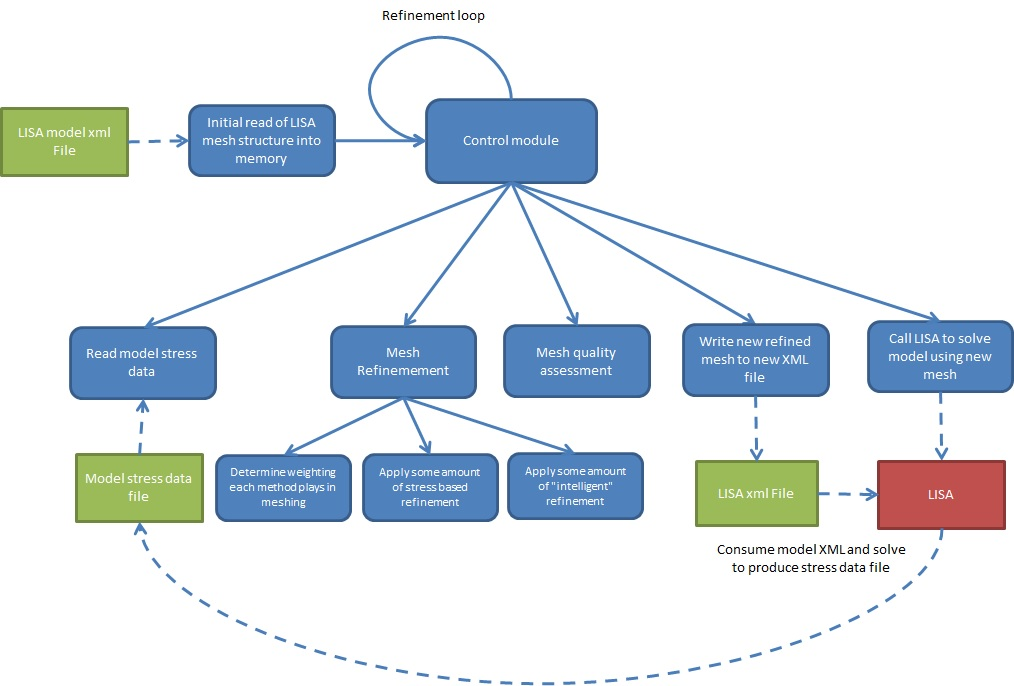
\includegraphics[width=150mm, scale=1]{../Graphics/SystemDesignDiagram.jpeg}}
  \caption{High level design of the system with its different modules}
  \label{fig:h-refinementImp}
\end{figure}


\subsection{Modular Architecture}
The modular architecture was crucial for allowing meshing algorithms and quality metrics to be replaced as necessary. At best the quality of the output could could only be predicted for each method before it was integrated into the system and executed in a range of different scenarios. To have tightly coupled these individual components would have rendered the overall system a failure in the event that any one of them failed. Instead the loose coupling of the architecture has enabled the system to be considered as more of a framework for testing the effects of combining different meshing approaches in order to generate a hybrid method.\\

\noindent
Although the system was highly modular It was also still desirable to maintain an architecture hierarchy so that classes could be developed independently but easily integrated. Composition was therefore generally favoured over inheritance as a means of building the architecture. Static classes and methods were also used when needing to write utility functions that were required by multiple high level subsystems and therefore did no fit especially well into any particular one. Examples of these are generic vector algebra operations such as dot product, matrix determinant and calculating surface normals.

\noindent
At the highest level namespaces were used to break down the class groups appropriately, namespaces also naturally structured as folders within the Visual Studio (VS) solution explorer (see appendix D) which made navigating the project and finding components much easier as the system expanded in size.

%\subsection{Mesh improvement Loop}
%As with many optimisation problems the refinement process is driven iteratively through a loop. Within the main loop all %interfacing with LISA, Mesh refinement and analysis is conducted which results in an updated version of the model that can be %handed to the subsequent iteration.


\subsection{Simulation Data Model}
Writing an API for LISA was the first stage of development for my project for which a design had to be considered. The API was crucial in order to program the more complex aspects using basic operations and avoid having to regularly perform direct string manipulation of the input files in order to manipulate the model. \\

\noindent
When the first re-meshing iteration occurs the system needs to read the input .liml file into an equivalent class model which closely resembles the files schema, diagrams for which can be seen in figure 4 below. Each class in this model contains corresponding data and methods used to represent and manipulate the model. These methods are then used by each of the refinement approaches to easily alter the mesh in a controlled manner. Once the mesh  has been adapted however it is required to be assessed by the modules responsible for validating its quality before finally being written back to a .liml file for LISA to solve on the subsequent iteration. Designing the data model so that it closely resembled the LISA scema not only made the higher level programming less confusing but also made serialisation of the data back to .liml format much simpler  thus reducing the number of bugs arising from inconsistencies between different representations of the same data. \\

\begin{figure}[h!!]
\centering
\begin{subfigure}{.5\textwidth}
  \centering
  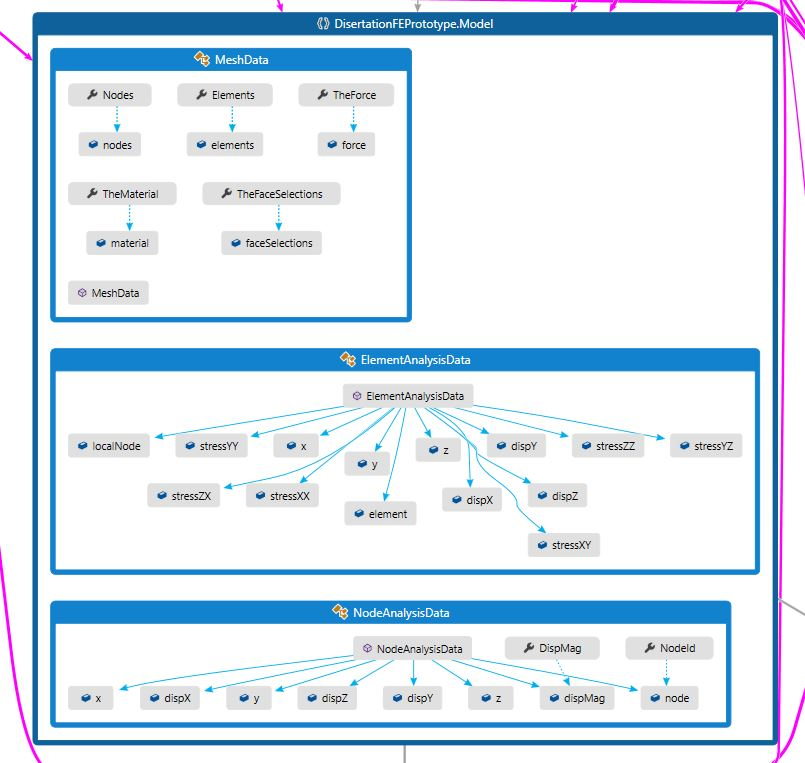
\includegraphics[width=0.9\linewidth]{../Graphics/DissoFEProto-Model.jpg}
  \caption{Model classes}
  \label{fig:sub1}
\end{subfigure}%
\begin{subfigure}{.5\textwidth}
  \centering
  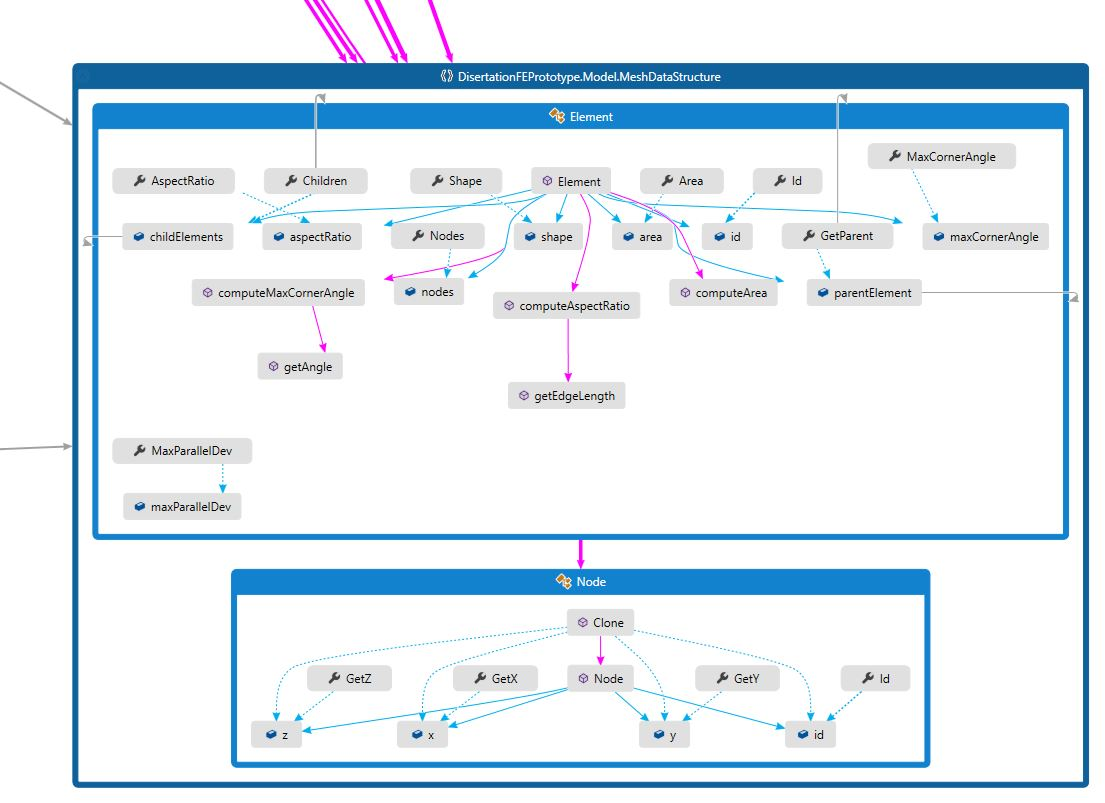
\includegraphics[width=0.9\linewidth]{../Graphics/DissoFEProto-ElemNode.jpg}
  \caption{Element and Node classes}
  \label{fig:sub2}
\end{subfigure}
\label{fig:test}
\end{figure}

\begin{figure}
\centering
\begin{subfigure}{.5\textwidth}
  \centering
  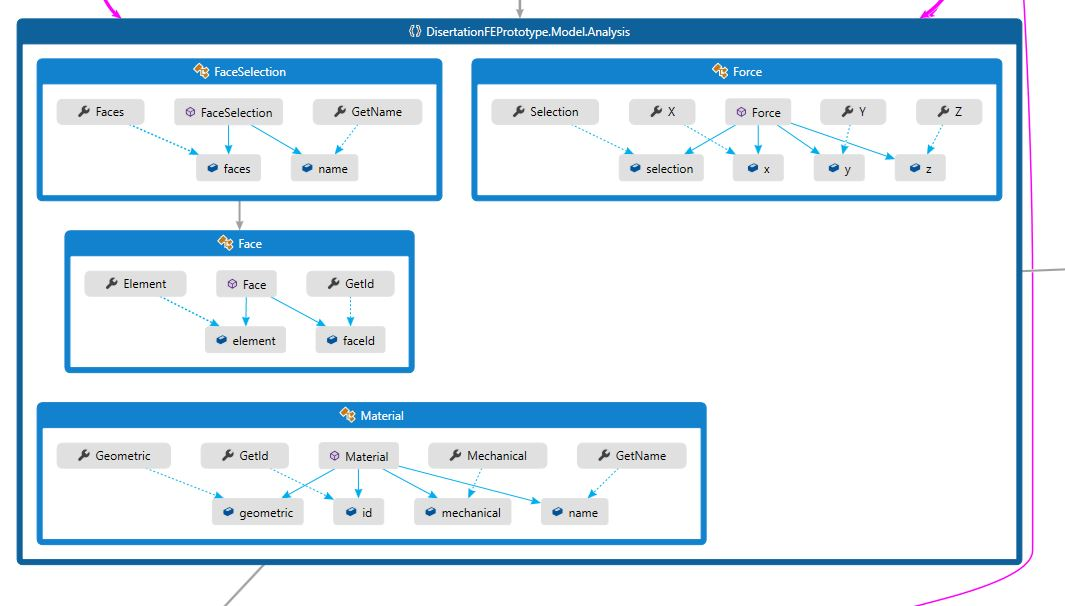
\includegraphics[width=0.9\linewidth]{../Graphics/DissoFEProto-ModelAnalysis.jpg}
  \caption{Model Analysis classes}
  \label{fig:sub1}
\end{subfigure}%
\begin{subfigure}{.5\textwidth}
  \centering
  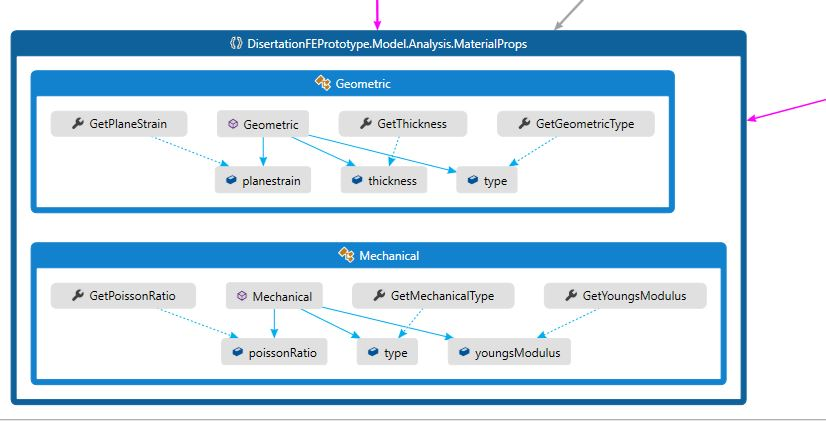
\includegraphics[width=0.9\linewidth]{../Graphics/DissoFEProto-MaterialProps.jpg}
  \caption{Material Property classes}
  \label{fig:sub2}
\end{subfigure}
\label{fig:test}
\caption{Class model to represent .liml file structure used by LISA}
\end{figure}

\noindent
One aspect of the data models design which greatly adds to the systems flexibility is the hierarchical design for representing the various Element types. At the root of this structure is the IElement interface, all new Element types must adhere to this in order for the various refinement methods to request refinement of an element using its class. Implementing the interface are a range of abstract classes such as ``SquareBasedElem" and ``TriangleBasedElem" These classes are designed to contain methods that are generally applicable for calculating metrics and re meshing individual elements where the elements fit this abstract category but their concrete implementation specifies their dimensionality and number of nodes, see Figure 6. This is powerful since computing metrics and performing subdivision for a 3d element is simply a reduction using the code for a 2D element but over every face comprising the 3D one. \\ 

\begin{figure}[h!!]                                                   
  \centerline{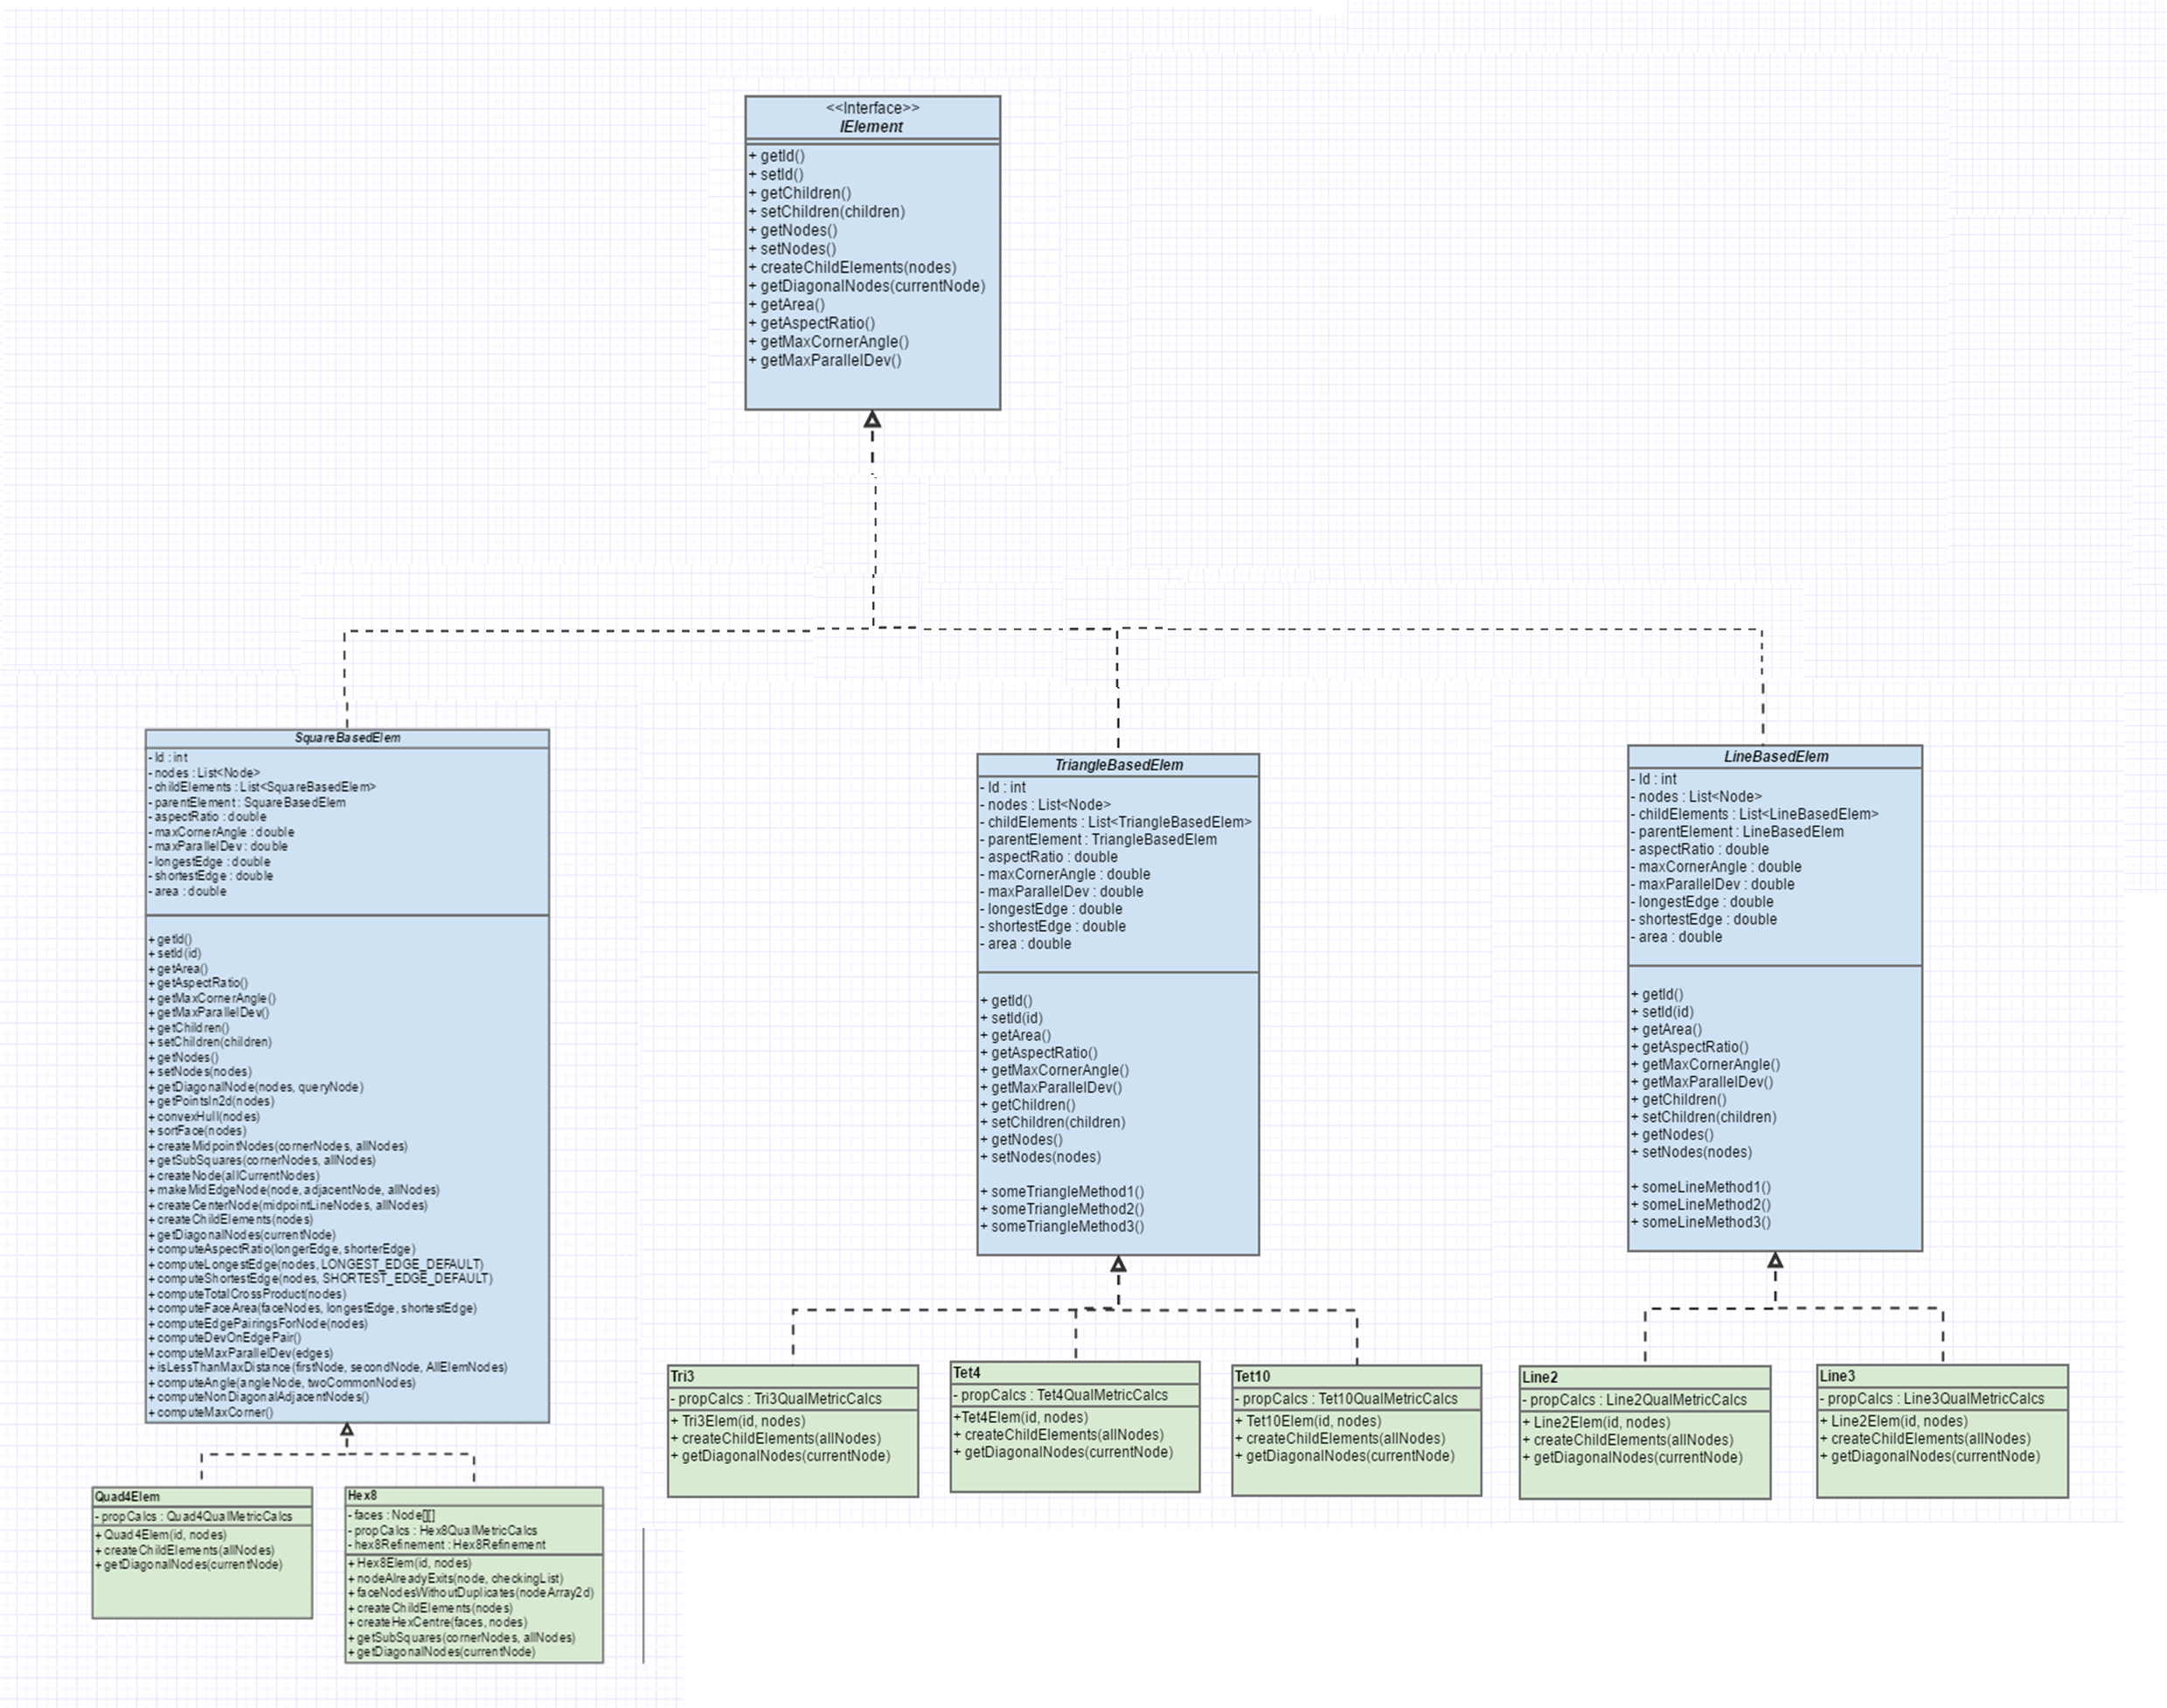
\includegraphics[width=150mm, scale=1]{../Graphics/ElementHigerarchyDiagram2.png}}
  \caption{Class diagram showing the hierarchy of element classification within the data model, due to time limitations I was not able to implement the respective classes for triangle and line based elements, to see image representations of each element type within this class diagram refer to element type appendix}
  \label{fig:h-refinementImp}
\end{figure}


\subsection{Remeshing methods approach}

Delegating refinement of individual elements to their respective classes made it much easier to decouple both the stress and heuristic methods allowing each of them to simply have the task of selecting elements which they considered beneficial to refine before calling the createChildElements() method on that element through the IElement interface. This allowed both of these high level refinement approaches to utilise the same low level functionality thus greatly improving code reuse and simplifying the design such that the high level meshing methods are relatively concise. \\

\noindent
Having reviewed both h-refinement \cite{HandPRefinements} and r-refinement \cite{RRefinement} as techniques for performing element subdivision it was concluded h-refinement was prefferable due to its simplicity and widespread use despite typically being more computationally expensive than r-refinement \cite{HandPRefinements} \cite{RRefinement}. \\ \\ \\ \\ \\

\noindent
Upon finishing subdivision and producing new child elements stored within their parents the refinement process also needed to flatten each tree to produce a new set of model elements. This task involved the deletion of parent elements and therefore needed to be performed by the ``OptimisationManager'' class responsible for combining and executing both refinement methods. \\

\noindent
Having evaluated a variety of approaches from the domains of AI it was concluded that the best approach for delivering a system capable of meeting the requirements and demonstrating effectiveness of a hybrid method would be an implementation of the heuristic expert system described by Dolsak. \\ 

\noindent
One key strength of selecting this approach as the alternative method by which to mesh was clear separation of the underlying AI method from what had to be implemented. This not only meant that focus could be given towards the design, implementation and evaluation of the general purpose system but demonstrated that the meshing procedure can for the most part be interchanged depending on the specific type of finite element analysis. \\ 


\subsection{Input Files}
The system requires three basic input files which should be placed within a directory that is given to the program as a parameter, these are files are:

\begin{itemize}
\item A structural model represented as a .liml file which LISA can solve.
\item An initial stress data file generated manually so the system has a starting point.
\item A JSON file containing important edges and associated meta data as identified by an engineer looking at the model.
\end{itemize}

An example of the content and format for each of these input files can be seen in Appendix B



\subsubsection{Combining methods}
Since each refinement method performed a discrete amount of subdivision every time it was called it made sense when developing a hybrid approach to simply enumerate the possible combinations for how much each method could be applied each iteration resulting in a set of two valued tuples up to some value :

\[ \left\{ (a, b) \,\middle|\, \, a,b \in \mathbb{N}\, \, a,b < k \right\} \]


\colorbox{yellow}{not sure if anyone actually cares about multithreading}

\noindent
Each tuple could then be considered one weighting configuration for combining the two methods and could be executed independent of the others to obtain a set of results for that weighting. Consequently it was possible to improve performance when conducting multiple evaluations through parallelism of the different weighting configurations as experiments onto independent threads. When started each thread creates its own directory which it copies the three input files to and runs for its designating weighting configuration. 


